

\begin{figure}[h!]
\center{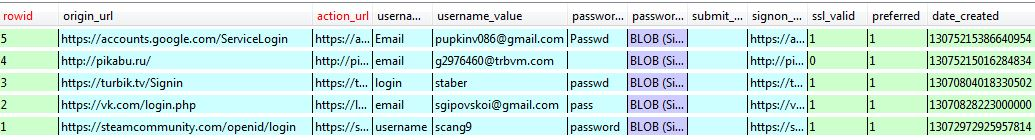
\includegraphics[width=0.7\linewidth]{ship_1}}
\caption{ Предыдущая версия интерфейса }
\label{ship_1:ship_1}
\end{figure}

\begin{figure}[h!]
\center{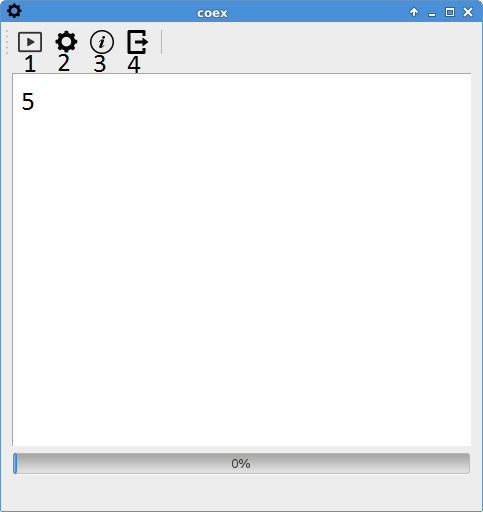
\includegraphics[width=0.7\linewidth]{ship_2}}
\caption{ Главное окно нового интерфейса }
\label{ship_2:ship_2}
\end{figure}

Новый интерфейс состоит из следующих элементов:
\begin{enumerate}
  \item элемент отвечающий за запуск coex;
  \item элемент отвечающий за настройки;
  \item сведения о программе;
  \item кнопка закрытия приложения;
  \item область вывода промежуточной информации.
\end{enumerate}

\begin{figure}[h!]
\center{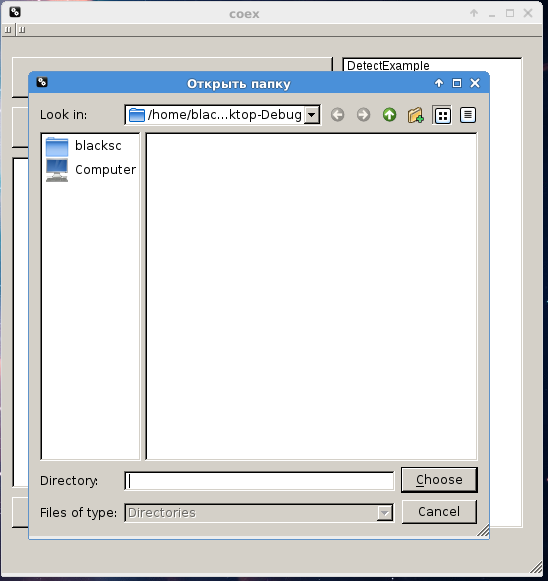
\includegraphics[width=0.7\linewidth]{ship_3}}
\caption{ Окно настроек }
\label{ship_3:ship_3}
\end{figure}

Интерфейс окна настроек состоит из следующих элементов:
\begin{enumerate}
  \item элемент <<исходная папка>> отвечает выбор папки, в которой будет производиться поиск;
  \item элемент <<папка назначения>> отвечает за выбор папки для сохранения результатов;
  \item данная область отвечает за выбор компонентов coex;
  \item элемент <<Сохранить>> отвечает за сохранения выбранных настроек.
\end{enumerate}

При следующем запуске приложения будут загружены сохраненные раннее настройки, а также геометрия главного приложения и его состояние т.е. оно откроется в том месте где его закрыли. Также данное окно является модальным т.е. оно прерывают работу главного окна и для продолжения его работы такое окно должно быть закрыто.

Для простоты мы предполагаем, что организация называется TUSUR, а приложение называется coex данные параметры прописываются в исходном коде приложения. Настройки будут храниться по-разному в зависимости от платформы.

  В системах Unix:
\begin{enumerate}
  \item HOME/.config/TUSUR/coex.conf;
  \item HOME/.config/coex.conf;
  \item /etc/xdg/TUSUR/coex.conf;
  \item /etc/xdg/TUSUR/.conf.
\end{enumerate}

  В Mac OS
\begin{enumerate}
  \item HOME/Library/Preferences/com.TUSUR.coex.plist;
  \item HOME/Library/Preferences/com.TUSUR.plist;
  \item /Library/Preferences/com.TUSUR.coex.plist;
  \item /Library/Preferences/com.TUSUR.plist.
\end{enumerate}

  В Windows настройки хранятся по следующим путям реестра:
\begin{enumerate}
  \item HKEY\_CURRENT\_USER\textbackslash Software\textbackslash TUSUR\textbackslash coex;
  \item <<HKEY\_CURRENT\_USER\textbackslash Software\textbackslash TUSUR>>;
  \item <<HKEY\_LOCAL\_MACHINE\textbackslash Software\textbackslash TUSUR\textbackslash coex>>;
  \item <<HKEY\_LOCAL\_MACHINE\textbackslash Software\textbackslash TUSUR>>.
\end{enumerate}
  

Содержание файла настроек представлено на рисунке~\ref{ship_25:ship_25}.

\begin{figure}[h!]
\center{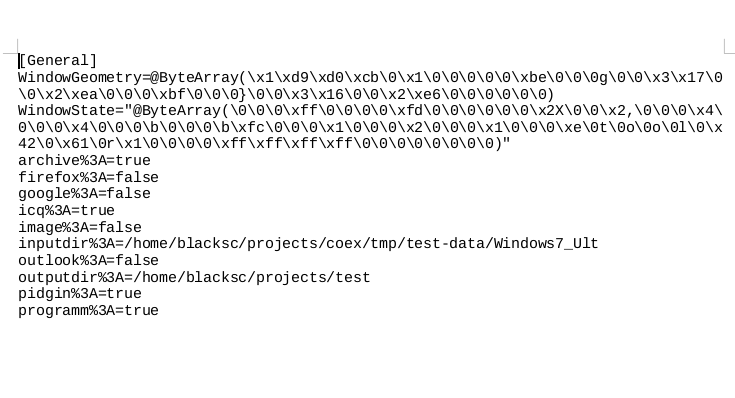
\includegraphics[width=0.9\linewidth]{ship_25}}
\caption{ Содержание файла настроек }
\label{ship_25:ship_25}
\end{figure}  

\begin{figure}[h!]
\center{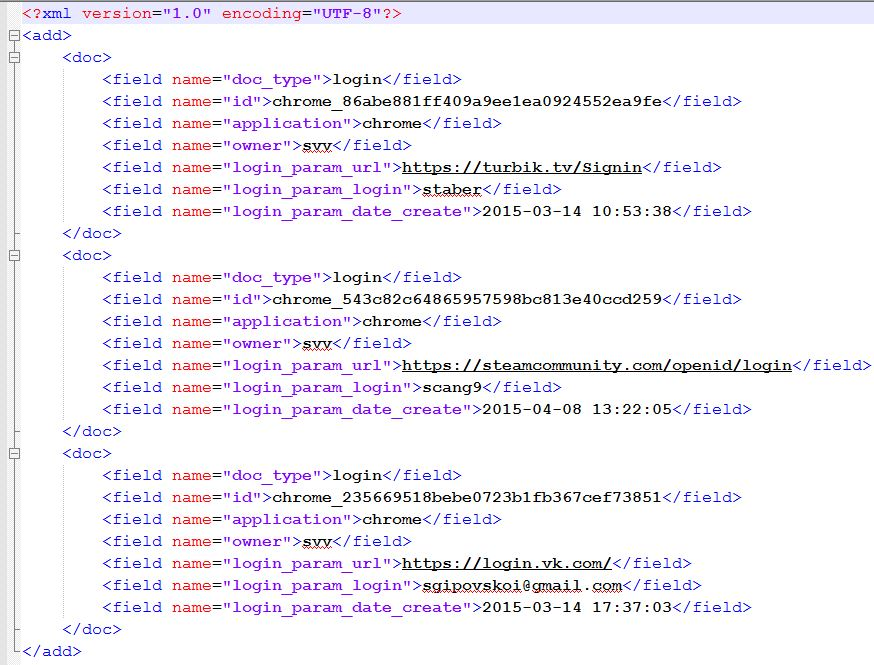
\includegraphics[width=0.7\linewidth]{ship_4}}
\caption{ О программе }
\label{ship_4:ship_4}
\end{figure}

\begin{figure}[h!]
\center{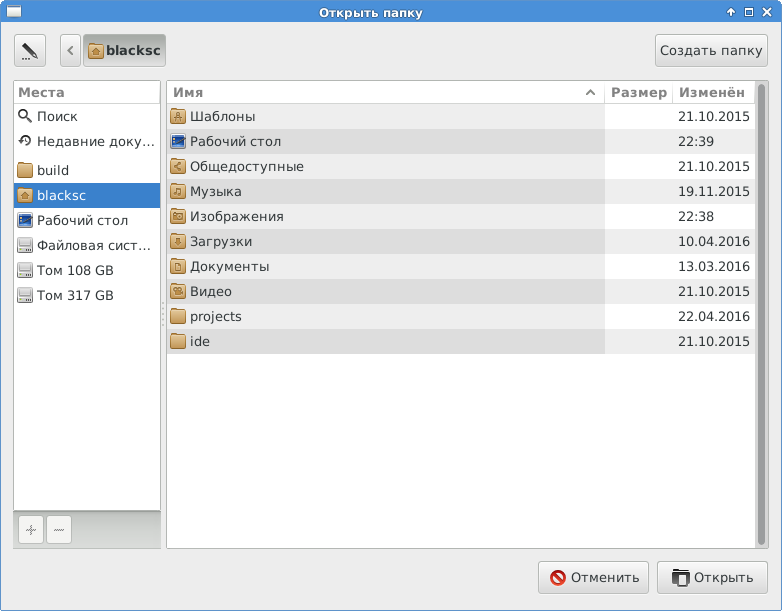
\includegraphics[width=0.7\linewidth]{ship_5}}
\caption{ Выбор директорий }
\label{ship_5:ship_5}
\end{figure}

Если не выбраны директории для работы, то при нажатии на кнопку “Запуск” отобразиться соответствующее сообщение (рисунок ~\ref{ship_6:ship_6}). Диалоговое окно выбора директории представлено на рисунке ~\ref{ship_5:ship_5}. По завершению работы системы отобразиться соответствующие сообщение (рисунок ~\ref{ship_7:ship_7}), при этом если нажать на кнопку “Результаты”, то откроется директория с результатами работы (рисунок ~\ref{ship_8:ship_8}).

\begin{figure}[h!]
\center{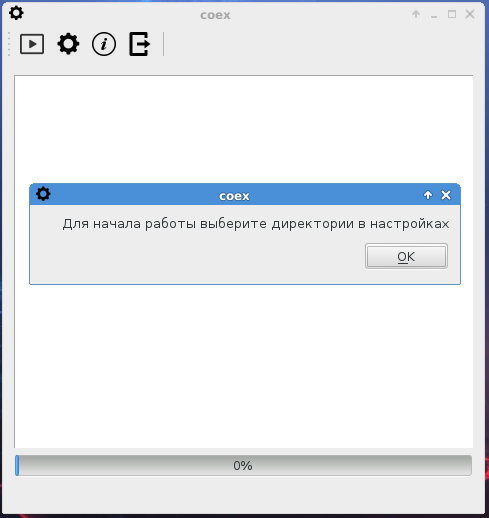
\includegraphics[width=0.7\linewidth]{ship_6}}
\caption{ Сообщение об ошибке }
\label{ship_6:ship_6}
\end{figure}

\begin{figure}[h!]
\center{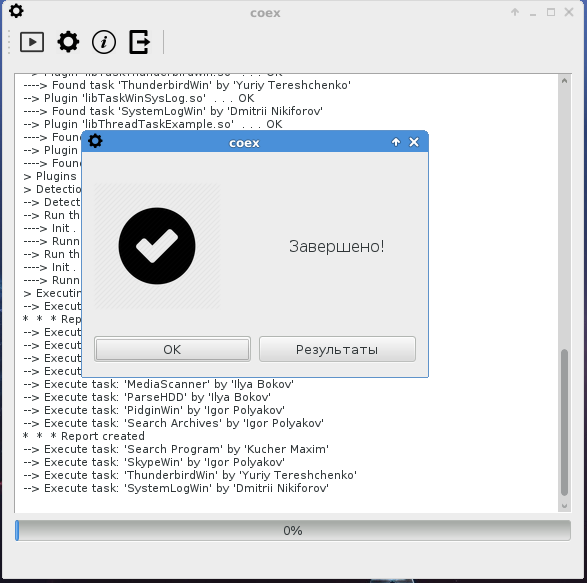
\includegraphics[width=0.7\linewidth]{ship_7}}
\caption{ Завершение работы }
\label{ship_7:ship_7}
\end{figure}

\begin{figure}[h!]
\center{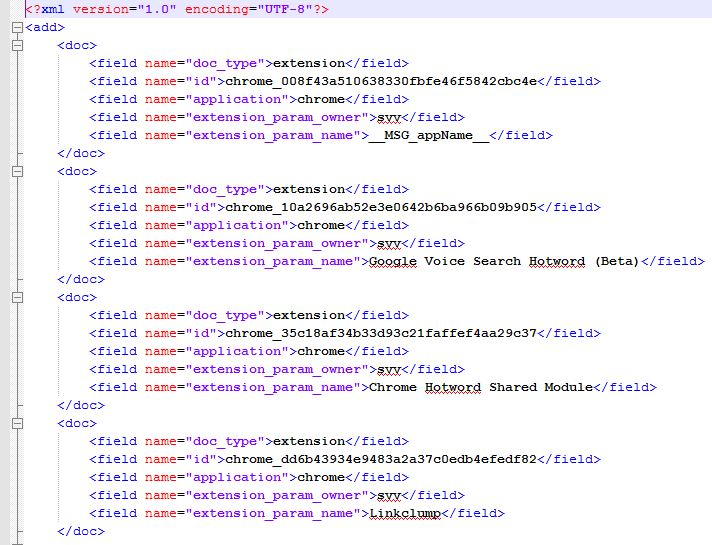
\includegraphics[width=0.7\linewidth]{ship_8}}
\caption{ Папка с результатами }
\label{ship_8:ship_8}
\end{figure}

\clearpage
